%!TEX root = Main.tex
\documentclass[Main]{subfiles}

\begin{document}

\section{Patterns used in the solution}
This section describes the different patterns used in this solution, and what they are used for.
\subsection{Wrapper Façade}
With Wrapper Façade you can encapsulate the basic C functions from the Operating System, and provide a Object Oriented Interface you can use instead.\\
Because it's an Interface without connection to the underlying OS, it can be implemented on multiple platforms and thereby enabling using the same interface no matter the platform.\\
This can speed up the development process, because the modules can be reused in different projects, and the application code isn't dependent on OS specific code.
\subsection{Reactor}
A Reactor can handle multiple requests from clients to a single application.\\
It collects the requests, Demultiplexes and executes them in a synchronous manner.\\
Because the Reactor executes events on a single thread, there will be no concurrency concerns. Class diagram for the reactor incorporating bridge and singleton patterns is shown in figure \ref{fig:reactoruml}.

\begin{figure}[hbtp]
\centering
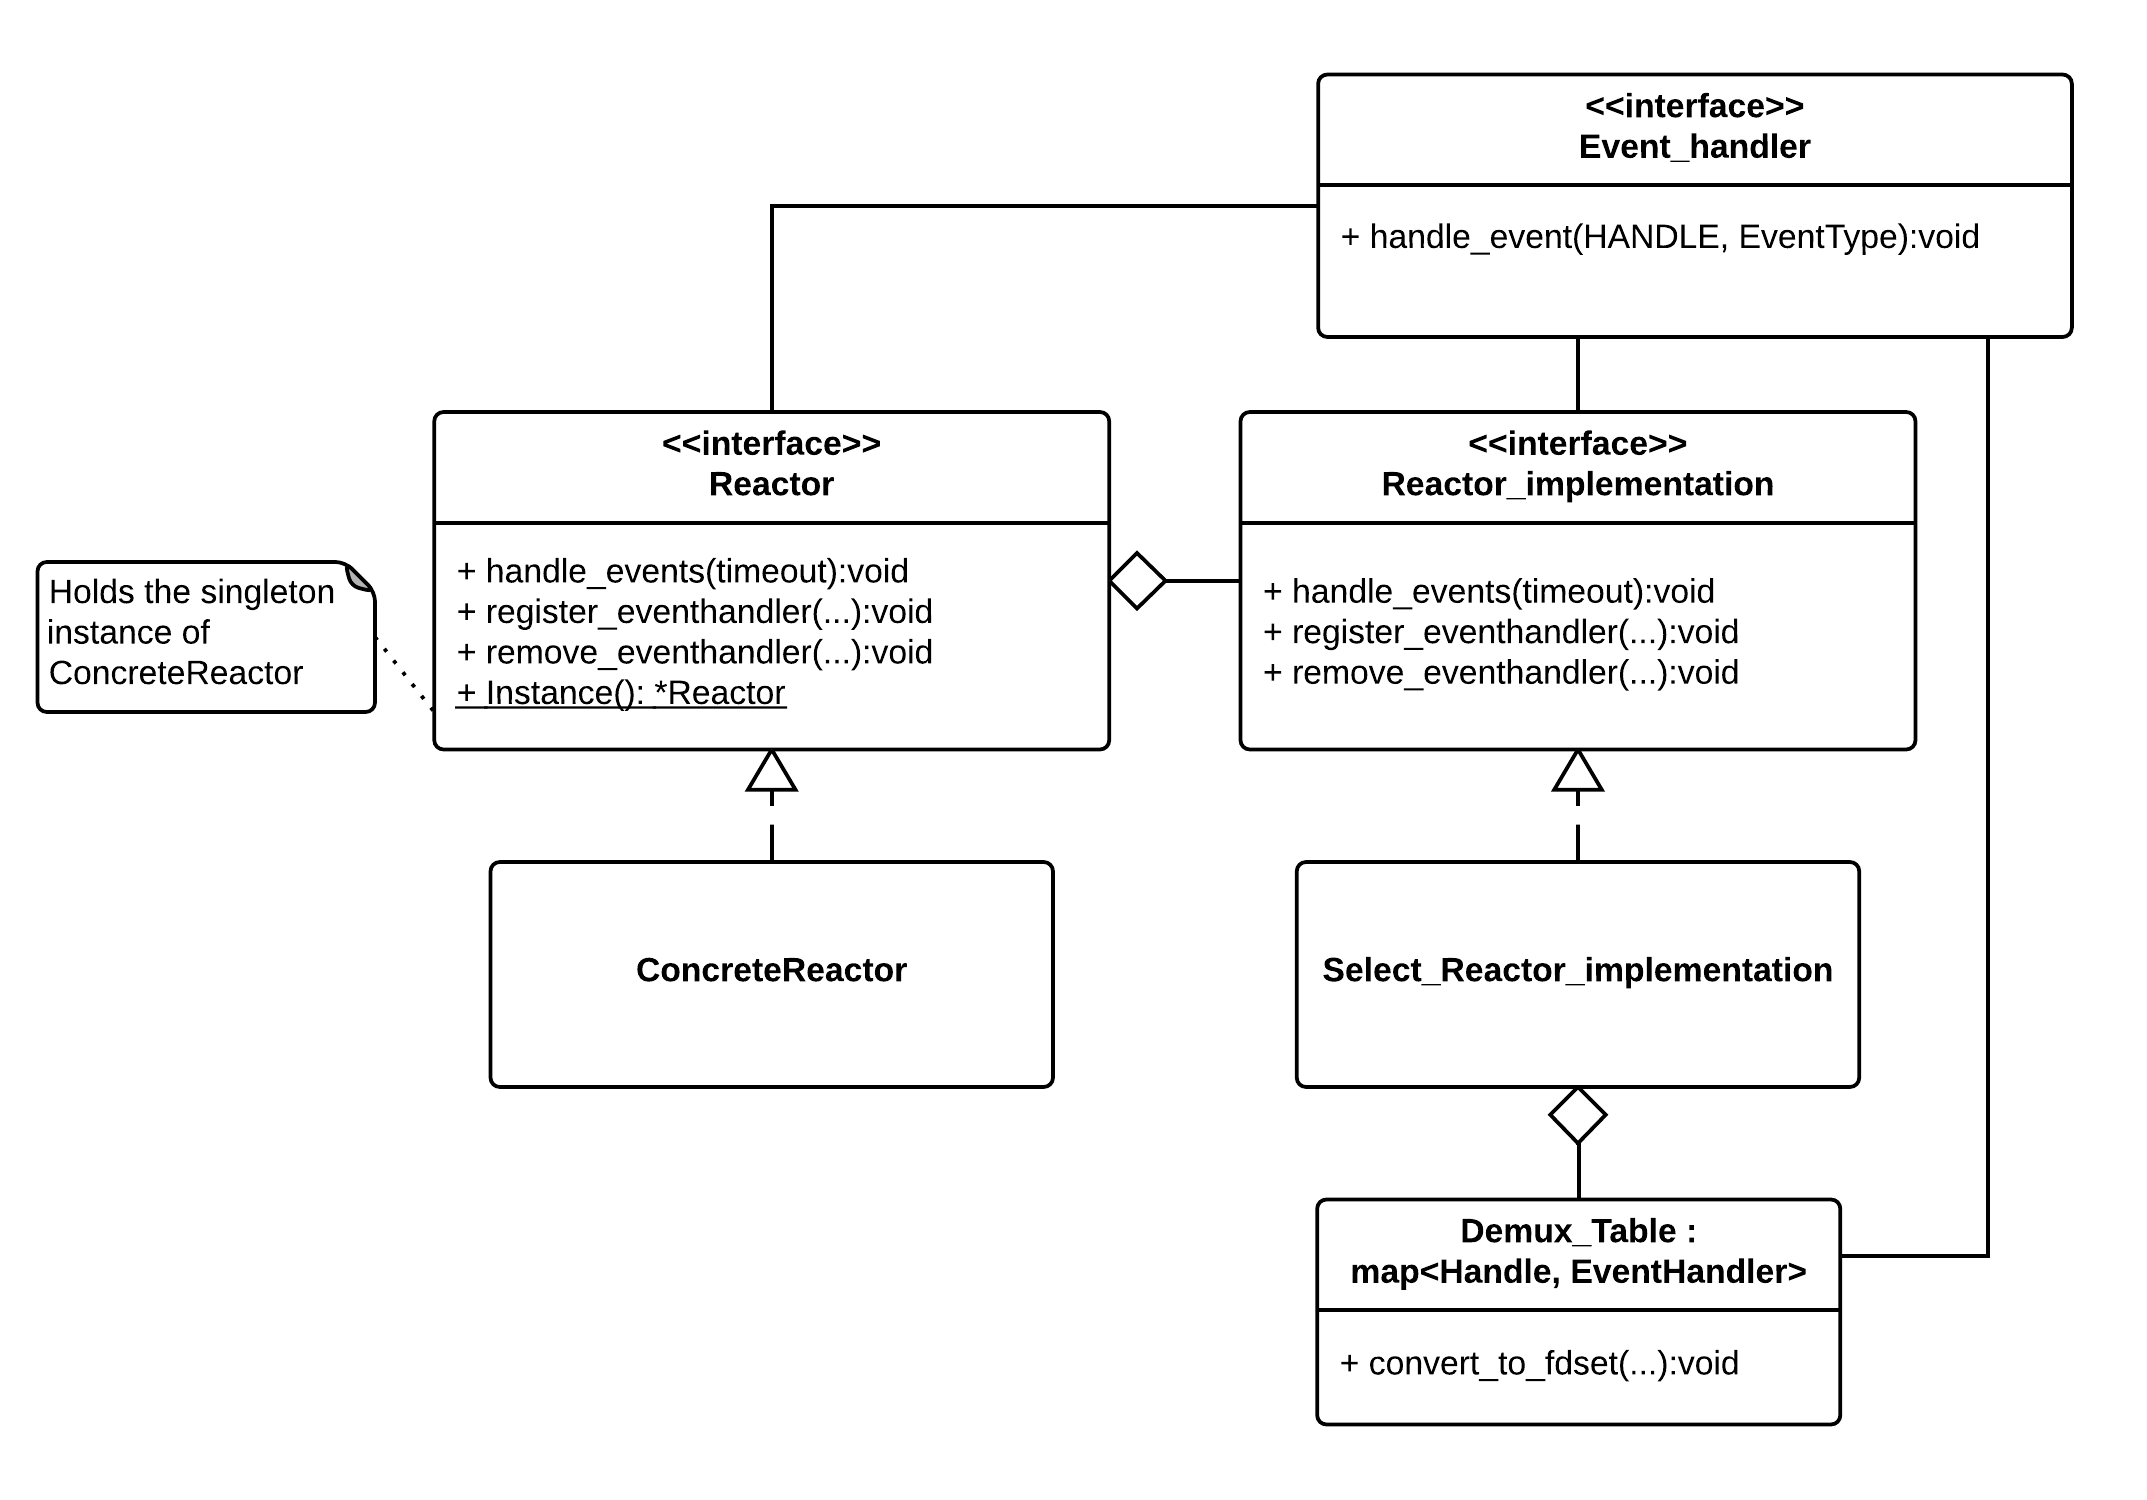
\includegraphics[width=1.0\textwidth]{exercise1reactor}
\caption{Class diagram for reactor incorporating bridge and singleton patterns.}
\label{fig:reactoruml}
\end{figure}

\subsection{Connector / Acceptor}
By encapsulating the initialization code, the Application code will be cleaner, and the action of creating a Client / Server design can be massively simplified.\\
When using the Connector / Acceptor pattern, the network initialization is hidden, and the application can focus on the tasks at hand.
This also gives a higher re usability and a lower coupling with the application.\\
This can be used together with the \code{Reactor}, to ensure the incoming requests are performed synchronous. 
\subsection{Bridge Pattern}
Used to create a gap between the abstraction and the implementation of a framework.\\
The functional implementations can then be created with Polymorphism. Class diagram for the reactor incorporating bridge and singleton patterns is shown in figure \ref{fig:reactoruml}.

\subsection{Singleton}
To ensure only a single instance of the object exists, it can be converted into a Singleton.
By hiding the constructor and only make it accesable via a static function, the object can be created, and reused for the duration of the application. This gives the benefit of every other object can access the same instance and modify it's data.\\
In this solution it have been used together with the \code{Reactor}. Class diagram for the reactor incorporating bridge and singleton patterns is shown in figure \ref{fig:reactoruml}.

\end{document}